\section{Hardware}
\subsection{FLYSKY Receiver}
The FLYSKY receiver is a compact wireless communication module used in remote-controlled systems to receive control signals from a FLYSKY transmitter. It operates on a 2.4GHz frequency band and supports multiple channels, allowing it to control various actuators such as motors and servos. This receiver is widely used in drones, RC planes, and robots due to its reliable range, low latency, and compatibility with many FLYSKY models. It typically connects directly to a flight controller or electronic speed controller (ESC) for signal routing.

\subsection{30A ESC Skywalker}
The 30A Skywalker ESC (Electronic Speed Controller) is a device designed to control the speed, direction, and braking of a brushless motor. Rated for a maximum continuous current of 30 amps, it is ideal for medium-sized electric drones and RC aircraft. It takes signals from the receiver or flight controller and converts them into three-phase power for the motor, allowing smooth acceleration and precise speed control. The ESC also includes safety features like overheating and overcurrent protection.

\subsection{Flight Stabilizer (NXE4 EVO)}
The NXE4 EVO Flight Stabilizer is an advanced control system used in RC aircraft and drones to maintain stability during flight. It uses onboard sensors such as gyroscopes and accelerometers to detect orientation and movement, and then automatically adjusts control surfaces or motor speeds to correct any deviations. This improves flight performance, especially in windy or unstable conditions, and enables smoother operation for both beginners and experienced pilots. It's essential for autonomous or semi-autonomous flight control.

\subsection{1000KV Brushless Motor}
A 1000KV brushless motor is a high-efficiency electric motor that rotates at 1000 revolutions per minute per volt applied. It is commonly used in drones, RC aircraft, and electric vehicles due to its power-to-weight ratio, reliability, and minimal maintenance needs. Unlike brushed motors, brushless motors have no internal contact between the rotor and stator, reducing wear and increasing lifespan. The motor typically has three wires for connection to an ESC and is paired with a propeller or gear mechanism for motion output.

\subsection{MG996 Metal Gear Servo}
The MG996 is a high-torque, metal gear servo motor used for precise angular movement in robotics, RC vehicles, and automation systems. Its durable metal gear construction offers increased torque and strength compared to plastic gear servos, making it suitable for demanding applications. Controlled by a PWM signal, it can rotate to specific angles between 0° and 180°, making it ideal for steering mechanisms, robotic arms, or flaps in RC aircraft. It comes with a standard 3-wire connector for power, ground, and signal.

\subsection{2200mAh 3S LiPo Battery}
The 2200mAh 3S LiPo (Lithium Polymer) battery is a high-capacity, lightweight power source commonly used in RC models, drones, and portable electronics. With three cells in series, it delivers a nominal voltage of 11.1V and a high discharge rate to support power-hungry components like motors and servos. Its 2200mAh capacity provides moderate runtime, making it ideal for short to medium-duration flights or robotic operations. The battery typically features a discharge plug (like XT60) and a balance connector for safe charging.

\subsection{Buck Module Voltage Regulator}
A buck module voltage regulator is a DC-DC converter that steps down higher input voltage to a lower, stable output voltage. It is commonly used in embedded electronics to power microcontrollers, sensors, and other 5V or 3.3V devices  from higher-voltage sources like LiPo batteries. The module includes components such as an inductor, capacitor, and adjustable potentiometer to maintain a consistent output. Its compact size and efficiency make it essential for battery-powered projects to protect components from over-voltage.

\subsection{Raspberry Pi with USB Camera and HDMI Cable}
The Raspberry Pi is a credit card-sized single-board computer capable of running a full Linux OS and performing various computing tasks. When paired with a USB camera, it can capture images and video for applications like computer vision, surveillance, and robotics. The HDMI cable allows video output to a monitor or display, enabling real-time viewing or debugging. This setup is ideal for lightweight, portable embedded systems where processing power, camera input, and display output are all required.
\begin{figure}
\centering
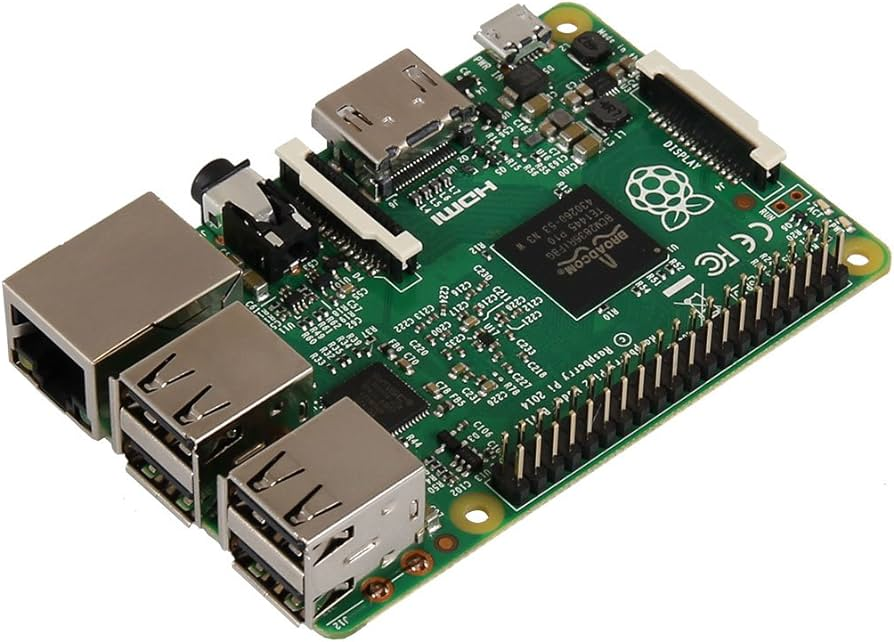
\includegraphics[width=0.5\textwidth]{images/raspimg.jpg}
\caption{Raspberry Pi 4 Model B}

\end{figure}
\section{Software}
\lipsum[4-8]
\section{Dataset}
\lipsum[4-8]
